\chapter{Orientation Estimation}
\label{ch:orientation_estimation}

In the motion monitoring field and especially in aircraft navigation the position of the coordinate frame of the body, with respect to a reference coordinate frame, is known as attitude, which is used as a synonym of orientation. There are different approaches to compute attitude estimates from magnetic and inertial data. This chapter explains their pros and cons and introduces sensor fusion as a means to mitigate the drawbacks of each approach. Before, two different ways of expressing orientation -- Euler angles and quaternions -- are described.

\section{Euler Angles}

Euler angles are one of several ways to describe the orientation of an object and its associated body frame in three-dimensional Euclidean space, with respect to the navigation frame, i.e. the reference frame. They represent a sequence of three elemental rotations about the axes of the coordinate system, defined as follows:

\begin{itemize}
\item The \emph{roll} angle $\phi$ determines the rotation around the $x$-axis with a range $-\pi < \phi \leq \pi$.
\item The \emph{pitch} angle $\theta$ determines the rotation around the $y$-axis with a range $-\frac{\pi}{2} \leq \theta \leq \frac{\pi}{2}$.
\item The \emph{yaw} angle $\psi$ determines the rotation around the $z$-axis with a range $-\pi < \psi \leq \pi$.
\end{itemize}

\noindent
Figure \ref{fig:Euler_angles} depicts the rotation about the axes $z, y^{'}, Z$ by $\psi, \theta, \phi$, respectively, according to the Tait-Bryan convention. The colour blue indicates the orientation before and the colour red the orientation after the rotation. In contrast to extrinsic rotations, where the three elemental rotations may occur either about the axes of the original coordinate system, the Tait-Bryan rotations are intrinsic rotations that occur about the axes of the rotating coordinate system, which changes its orientation after each rotation.

\begin{figure}[ht]
\centering
\begin{tikzpicture}[scale=1.4]
\node[inner sep=0pt] (tait) at (0,0)
    {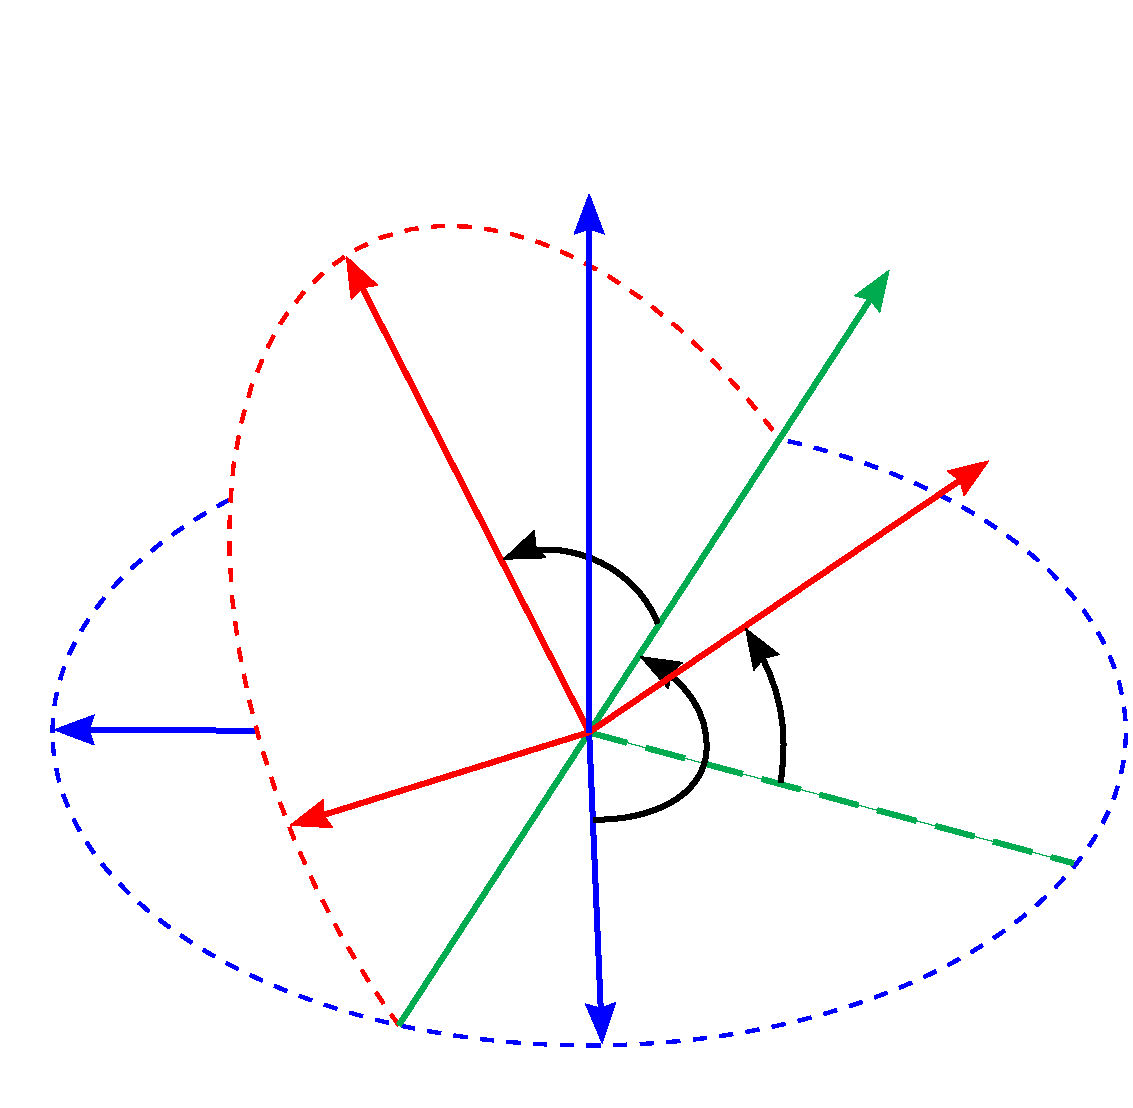
\includegraphics[width=.7\textwidth]{Images/taitbryan.pdf}};
    
\node [] at (0.5,0.2) {$\phi$};
\node [] at (0.65,-1.85) {$\psi$};
\node [] at (1.55,-0.9) {$\theta$};

\node [] at (-3.4,-1.1) {$x$};
\node [] at (0.25,-3.3) {$y$};
\node [] at (0.12,2.43) {$z$};
\node [] at (2.0,1.2) {$y^{'}$};


\node [] at (2.8,0.6) {$X$};
\node [] at (-1.5,2.05) {$Y$};
\node [] at (-2.0,-1.7) {$Z$};
\end{tikzpicture}
\caption{Representation of the body frame (red) with respect to the navigation frame (blue). The body frame was rotated, by the Euler angles $\psi, \theta, \phi$ about the axes $z, y^{'}, X$, respectively. Adapted from \cite{Wiki_taitbryan}.} \label{fig:Euler_angles}
\end{figure}

\section{Transformation Matrices}

Coordinates representing a point in one coordinate system can be transformed to another. Such a linear transformations can be expressed as multiplication of a matrix with the coordinate vector that is to be transformed. Let $\mathbf{E}$ denote the orthonormal basis $\{x, y, z\} \in \mathbb{R}^3$ and let $\mathbf{E}^{'}$ denote the orthonormal basis $\{X, Y, Z\} \in \mathbb{R}^3$. Furthermore, let $\mathbf{b}$ denote the position vector of a point in three-dimensional Euclidean space. The coordinate transformation from $\mathbf{E}$ to $\mathbf{E}^{'}$ is denoted $\mathbf{\Omega}_{\mathbf{E} \rightarrow \mathbf{E}^{'}}: (b_1, b_2, b3) \mapsto (b1^{'}, b2^{'}, b3^{'})$. Then, the transformation from $\mathbf{b}$ to $\mathbf{b}^{'}$ is given by

\begin{equation}\label{eq:transformation}
  \mathbf{b^{'}} = \mathbf{\Omega}_{\mathbf{E} \rightarrow \mathbf{E}^{'}}(\mathbf{b}) = \mathbf{T} \mathbf{b}\,,
\end{equation}

\noindent
where $\mathbf{T}$ is the transformation matrix. To transform the coordinate vector from the navigation frame to the body frame, according to the common aerospace rotation sequence mentioned above and the Nort-East-Down system (NED), the transformation matrix $C_{nb}$ is given by

\begin{equation}
\begin{split}
\mathbf{C}_{nb} & = \mathbf{T}_x(\phi) \mathbf{T}_y(\theta) \mathbf{T}_z(\psi) \\
 & = {\left[ \begin{smallmatrix}
    1 \; & 0 \; & 0 \\
    0 \; & \cos \phi \; & \sin \phi \\
    0 \; & -\sin \phi \; & \cos \phi
    \end{smallmatrix}\right]}
    {\bigg[ \begin{smallmatrix}
    \cos \theta \; & 0 \; & -\sin \theta \\
    0 \; & 1 \; & 0 \\
    \sin \theta \; & 0 \; & \cos \theta
    \end{smallmatrix} \bigg]}
    {\left[\begin{smallmatrix}
    \cos \psi \; & \sin \psi \; & 0 \\
    -\sin \psi \; & \cos \psi \; & 0 \\
    0 \; & 0 \; & 1
    \end{smallmatrix}\right]}\\
 & = {\left[\begin{smallmatrix}
   \cos \theta \cos \psi \; &
    \cos \theta \sin \psi \; &
   -\sin \theta \\
    \sin \phi \sin \theta \cos \psi - \cos \phi \sin \psi \;\; &
    \sin \phi \sin \theta \sin \psi + \cos \phi \cos \psi \;\; &
    \sin \phi \cos \theta \\
    \cos \phi \sin \theta \cos \psi + \sin \phi \sin \psi \;\; &
    \cos \phi \sin \theta \sin \psi - \sin \phi \cos \psi \;\; &
    \cos \phi \cos \theta
  \end{smallmatrix}\right]}
\end{split}
\end{equation}

\noindent
Plugged in Equation \ref{eq:transformation} ($\mathbf{T} = \mathbf{C}_{nb}$) the left multiplication of the matrices $\mathbf{T}_x(\phi), \mathbf{T}_y(\theta), \mathbf{T}_z(\psi)$ to the vector $\mathbf{b}$ represent the orthogonal projection onto the axis of the coordinate system that result from the two-dimensional rotation of $\phi, \theta, \psi$ about the axes $x, y, z$, respectively. The matrix $\mathbf{C}_{bn}$ for transforming the coordinate vector from the body frame to the navigation frame is given by

\begin{equation}
\mathbf{C}_{bn} = {\left[\begin{smallmatrix}
   \cos \theta \cos \psi \; &
    \sin \phi \sin \theta \cos \psi - \cos \phi \sin \psi \; &
    \cos \phi \sin \theta \cos \psi + \sin \phi \sin \psi \\
    \cos \theta \sin \psi \;\; &
    \sin \phi \sin \theta \sin \psi + \cos \phi \cos \psi \;\; &
    \cos \phi \sin \theta \sin \psi - \sin \phi \cos \psi \\
    -\sin \theta \;\; &
    \sin \phi \cos \theta \;\; &
    \cos \phi \cos \theta
  \end{smallmatrix}\right]}
\end{equation}

\noindent
The matrices $\mathbf{C}_{bn}$ and $\mathbf{C}_{nb}$ are known as Direct Cosine Matrices. Note that $\mathbf{C}_{bn} = \mathbf{C}^T_{nb} = \mathbf{C}^{-1}_{nb}$, so that $\mathbf{C}^{ }_{bn} \mathbf{C}_{nb} = \mathbf{I}$.  

\section{Quaternions}

\section{Projection of Gravity Vector and Earth's Magnetic Field Vector}

As described in Chapter \ref{ch:MARG}, accelerometers measure the acceleration they experience. Under static or quasi-static (steady, linear motion) conditions, or at low acceleration it can be assumed that the measured acceleration is mainly that of gravity. Be means of simple trigonometric transformations estimates for the pitch and the roll angle can be obtained. Since the gravity vector is perpendicular to the $xy$-plane and thus a rotation around the $z$-axis will not cause any variation in the sensed acceleration, the yaw angle cannot be obtained by this method. To solve this problem a three-dimensional magnetometer is used, which measures the variation of Earth's magnetic field while rotating around the $z$-axis.

\section{Integration of Angular Rate}

Another way to estimate the attitude of an object is the integration of the angular rate around the $x, y$ and $z$-axis, respectively. Although this would theoretically lead to very accurate orientation estimates, they are impaired by \gls{ARW} and dynamical bias in practice. \gls{ARW} is an effect caused by the integration of high-frequency, thermo-mechanical noise, which leads to a random additive angle in the orientation signal. An even greater impact than AWR has the gyroscopes dynamic bias, which has its origin in low-frequency flicker noise. Both effects cause a dramatical drift in the angle signal over time.

\section{Sensor Fusion}

Since the projection of the gravity vector and the Earth's magnetic field vector are only valid under static or quasi-static conditions, or at low acceleration, and the integration of the angular rate leads to non-reliable estimates due to suffering from \gls{ARW} and dynamic bias, but is not affected by the intensity of motion, a means to combine the information of both sensors is desirable. The combination of information from multiple sensors to increase the overall precision of the estimation of a certain quantity of interest is termed sensor fusion. \citeauthor{raol2009multi} \cite{raol2009multi} states the following advantages of sensor fusion:
 
\begin{itemize}
\item Robust functional and operational performance is given, in case of data loss from one sensor, due to redundancy provided by multiple sensors.
\item Enhanced confidence in the results inferred from the measurement of one sensor, if they are confirmed by the measurement of another sensor.
\item With sensor fusion an arbitrary fine time resolution of measurements is possible, whereas single sensors need a finite time to transmit measurements and so limit the frequency of measurements.
\item One sensor might be, to some extent, better in a certain state of the measured process, e.g. low or high motion intensity in attitude estimation, and thus, by fusing multiple sensor signals, a satisfactory accuracy among all states of the process could be attained.
\end{itemize}

\noindent
Sensor fusion can be realised by the use of a Kalman filter, which is described in detail in the next chapter.


